\documentclass[a4paper,12pt]{article}
\usepackage[utf8]{inputenc}
\usepackage{geometry}
\usepackage{graphicx}   % images
\usepackage{fancyhdr}   % headers/footers
\usepackage{tcolorbox}
\usepackage{listings}
\usepackage{xcolor}
\geometry{margin=1in}

% ---------- Header ----------
\setlength{\headheight}{36pt}
\setlength{\headsep}{18pt}
\renewcommand{\headrulewidth}{0.4pt}
\fancyhf{}
\fancyhead[L]{
\includegraphics[width=0.13\textwidth, keepaspectratio]{Figures/UM6Plogo.png}}
\fancyhead[R]{
\includegraphics[width=0.13\textwidth, keepaspectratio]{Figures/CC.jpg}}
\fancyfoot[L]{Data Management Lab}
\fancyfoot[R]{Prof. Karima Echihabi}
\fancyfoot[C]{Page \thepage}

% ---------- Deliverable Template ----------
\begin{document}
\thispagestyle{empty}
\begin{center}
  
\includegraphics[width=0.25\textwidth]{Figures/UM6Plogo.png}\hfill
  
\includegraphics[width=0.25\textwidth]{Figures/CC.jpg}
  \vspace{1.2cm}

  {\LARGE \textbf{Deliverable \#: Conceptual Design}}\\[0.6cm]
  {\large \textbf{Data Management Course}}\\[0.2cm]
  {\large UM6P College of Computing}\\[0.8cm]

  {\normalsize \textbf{Professor:} Karima Echihabi \quad 
   \textbf{Program:} Computer Engineering}\\[0.1cm]
  {\normalsize \textbf{Session:} Fall 2025}\\[1cm]

  \rule{0.9\textwidth}{0.5pt}\\[0.5cm]
  {\large \textbf{Team Information}} \\[0.3cm]
  \begin{tabular}{|l|l|}
    \hline
    \textbf{Team Name} & QueryMaster \\ \hline
    \textbf{Member 1}  & El Mehdi Regagui  \\ \hline
    \textbf{Member 2}  & Yasser Jarboua   \\ \hline
    \textbf{Member 3}  & Adam Ibourg-EL Idrissi   \\ \hline
    \textbf{Member 4}  & Salma Mana   \\ \hline
    \textbf{Member 5}  & Hiba Mhirit   \\ \hline
    \textbf{Member 6}  & Sara Qiouame   \\ \hline
    \textbf{Member 7}  & Douaae Mabrouk   \\ \hline
    \textbf{Repository Link} & \texttt{https://github.com/yasserJarboua/QueryMasters/} \\ \hline
  \end{tabular}
  \rule{0.9\textwidth}{0.5pt}\\
\end{center}
\clearpage
\pagestyle{fancy}

% ---------- Sections for Students ----------
\section{Introduction}
The Moroccan National Health Services (MNHS) requires a special database design in order to support their services, with the aim to manage patients, staff, hospitals, departments, appointments, prescriptions, medications, insurance, billing, and emergencies.The deliverable represents the conceptual design of the MNHS database using the ER diagram, showing the different relations and attributes that characterize each component of their environment. 

\section{Requirements}
The deliverable should represent clearly the relations between each  entity of the MNHS database, providing a full view of all the interactions, the participation constraints and the attributes of each entity and relation, all provided as an ER diagram.
\subsection{Requirements Details}
Our ER model addresses the following MNHS requirements:
\begin{itemize}
    \item Patients with internal ID, optional CIN, Full name, DoB, sex, blood group, phone and multiple contact locations(each including street, city province, postal code and an optional phone).
    \item Staff categorized into practitioners, caregivers, and technical staff with role-specific attributes.
    \item Hospitals and departments, where each department belongs to exactly one hospital.
    \item Appointments linking one patient, one staff member, and one department, with the track of date, time, reason and status(Scheduled, Completed, Cancelled).
    \item Prescriptions issued by staff to patients, including multiple medications with dosage and duration.
    \item Medications include: DrugID, name, form, strength, manufacturer, therapeutic, class and active ingredient.
    \item Insurance coverage (CNOPS, CNSS, RAMED, private, or none), allowing multiple insurances per patient.
    \item Billing attached to clinical activities and linked to one insurance.
    \item Emergencies
    \item Pharmacy inventory tracked per hospital and medication (quantity, reorder level, unit price).
\end{itemize}
\newpage
\section{Methodology}
In order to explain the design choices we will go through two sections: Entities Description and then the existing relations between them.
\subsection{Entities Description: }
\begin{itemize}
    \item Patients: we've chosen to represent the patient as an entity, we chose the internal identifier as the primary key on our design because not everyone has a (CIN), a patient could be an adult as he could be a child, which motivated us to keep CIN as an optional attribute.Concerning the contact locations we decided to model it as a separate entity linked to Patients. We assigned it an AddressID as the primary key, with attributes such as street, city, province, postal code, and optional phone.
    \item Staff: we used the ISA Hierarchies to describe the subclasses of the staff entity (Practitioner, caregiving, technical) recording for each of them the necessary attributes mentioned on Lab description, and an id attached to the staff attribute. 
    \item Hospitals And Departments: we chose to consider them both as entities, with a primary Key for each of them and with keeping track of their mandatory attributes (Hospitals: name, city, region / Departments: ).
    \item Medications: the drugID is considered as our primary key to this entity, different attributes are linked to it to record the medications characteristics (class, name, from ...)
    \item Insurance: it has the attribute coverage type that holds different values (CNOPS, CNSS, RAMED, OR None)
    \item Bills: identified by the billID
    \item Emergency: Considered as weak entity to patients, has the attributes admission timestamp, triage level(from 1(immediate) to 5(Non-Urgent)) and outcome;
\end{itemize}
\subsection{Relations Between the entities}
\begin{itemize}
    \item Patient Related Relationships:
    \begin{enumerate}
        \item Clinical Activities: it is a ternary relationship that links a patient, with at least a staff and bills, in the other hand a staff may have linked pair of patient and bills because not all the staff may do a clinical activity(like security guards etc...), and a bill has to have at least one patient and staffs we avoided using a bold arrow because many staff members may interact in one clinical activity.
        \item live-in : to match the patient with its appropriate contact location, each patient may have several contact locations which is described on the ER Diagram as a thin line between the patients and contact location. 
        \item Covers: It's a relation that links between a patient and an insurance, as in the lab description a patient can have more than one insurance.
        \item Appointments: We've chosen to represent it as a ternary relationship between Patient, Department and Staff.The usage of Bold arrows is justified by the constraint that the relation is between exactly one patient one staff and one department, and it records status, reason, time, date.
        \item Prescription: it's a ternary relation between patient, staff and medication, it's not a total participation because a prescription may not contain a medication.In addition it holds three attributes: dosage, duration and a date.
        \item undergoes: Links the patients with emergency as weak entity because its existence depends on patients existence.
    \end{enumerate}
    \item Staff Related Relationships:
    \begin{enumerate}
        \item Appointment: Already discussed on the Patients relations.
        \item Prescriptions: Already discussed on the Patients relations.
        \item Clinical Activities: Already discussed on the Patients relations.
        \item Take over: it links between staff and emergency and it's a partial relation because it is mentioned that it is optional to have a staff who handled the triage/attending. 
        \item WorK: it links between department and staff, a staff has to have at least one department to work on and a depart may have 0-many staffs,we did not add the relation ‘Assigned to’ because we considered it equivalent to the ‘Work’ relation.
    \end{enumerate}
    \item Department Related Relationships:
    \begin{enumerate}
        \item Appointment: Already discussed on the Patients relations.
        \item Belong: a department belongs exactly to one hospital which is described as a bold arrow on the relationship.
    \end{enumerate}
    \item Hospital Related Relationships:
    \begin{enumerate}
        \item belong: Already discussed on the Department relations.
        \item Pharmacy Inventory: links between medications and Hospital and keeps track for each hospital the on-hand quantity, reorder level, last restock timestamp,
and unit price per medication.
    \end{enumerate}
    \item Medications Related Relationships:
    \begin{enumerate}
        \item Prescription: Already discussed on Patients relations.
        \item Pharmacy Inventory: Already discussed on Hospital relations.
    \end{enumerate}
    \item Bills:
    \begin{enumerate}
        \item Clinical Activities: Already discussed on the patients relations.
        \item Linked to: each bill is only linked to exactly one
insurance, and an insurance has at least one bill.
    \end{enumerate}
\end{itemize} 
\section{Implementation \& Results}
\begin{figure}  % [p] forces it onto its own page
  \centering
  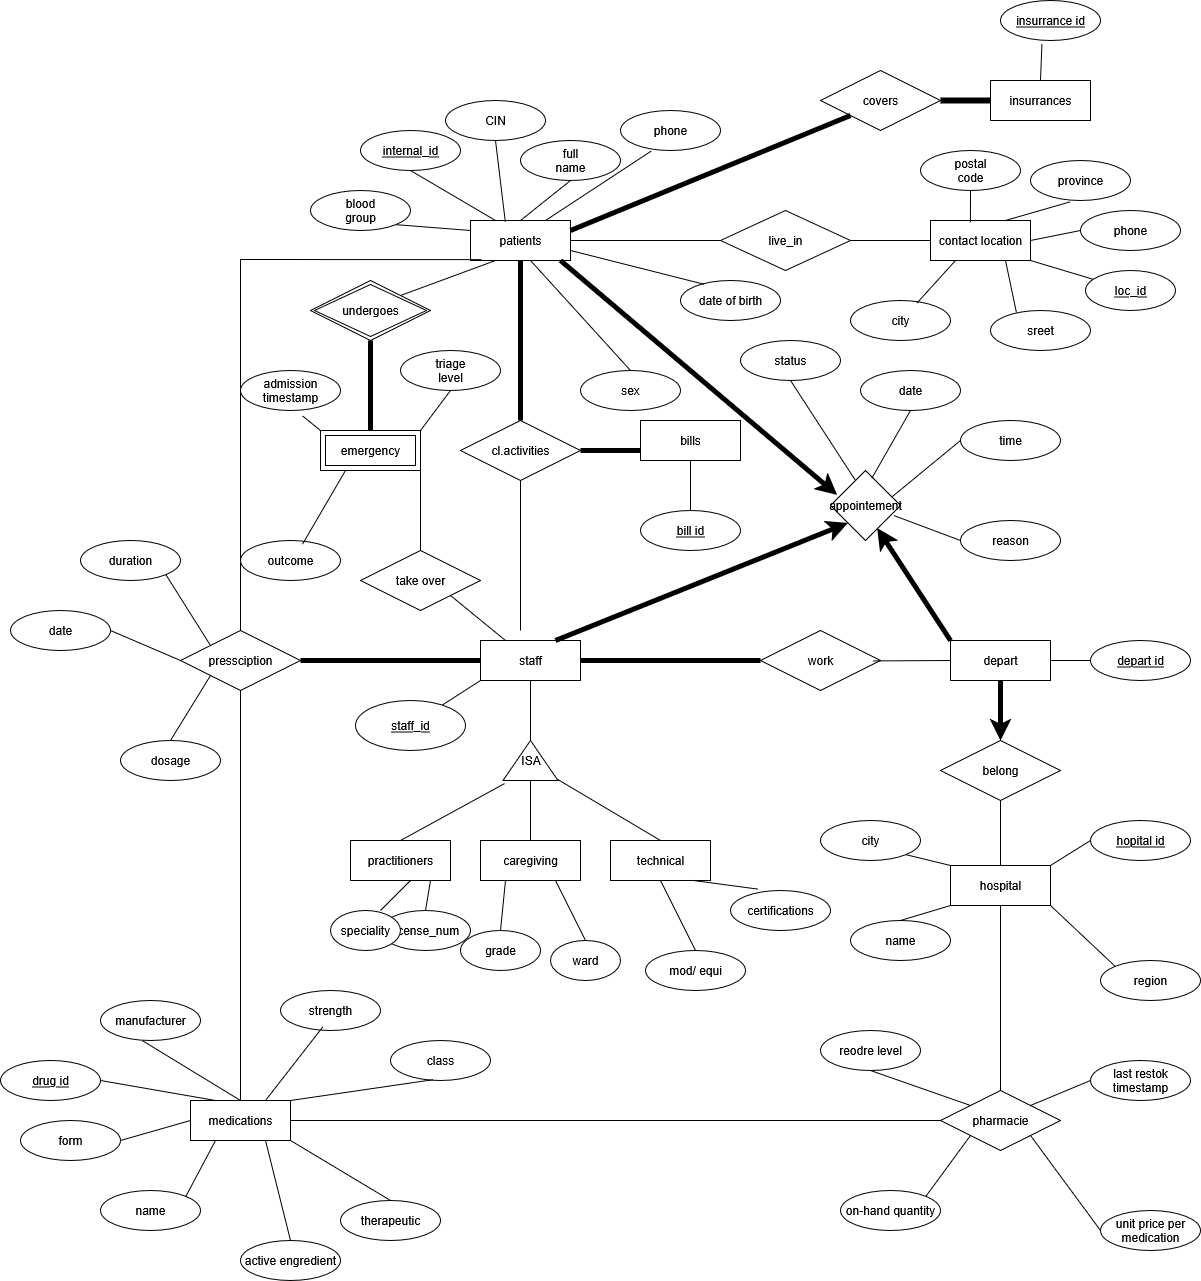
\includegraphics[width=\textwidth,height=\textheight,keepaspectratio]{Figures/ER Diagram.png}
  \caption{Entity–Relationship Diagram for MNHS Database}
  \label{fig:erd}
\end{figure}
\newpage

\section{Discussion}
\subsection{Challenges Faced During the Project:}
\begin{enumerate}
    \item Different Interpretations of Relationships:
Each team member understood the relationships mentioned in the script differently, which caused confusion and inconsistencies in our work.
    \item Confusion Around Ternary Relationships:
We struggled to fully grasp the concept of ternary relationships and when it is appropriate to replace them with aggregation.
    \item Optimization of the ER Model:
Towards the end, we were unsure whether we could add additional relationships or details to improve clarity and meaning, or if we had to strictly adhere to the original script without modifications. On one hand, refining the model could improve clarity and better convey our understanding. On the other hand, keeping it unchanged would preserve the authenticity of our initial interpretation and work. This dilemma made it challenging to decide how much to revise the model without losing the essence of our original efforts.
\end{enumerate}

\subsection{Lessons Learned:}

\begin{enumerate}
    \item We discovered how challenging it can be to precisely capture customer requirements when creating the ER model.
    
    \item We learned many new concepts about ER diagrams, especially when dealing with complex cases that required deep reflection and discussion.
    
    \item We began developing the intuition needed to choose the best modeling approach---whether to use ternary relationships, binary relationships, or aggregation.
    
    \item We improved our logical thinking skills by connecting real-world situations with the project content.
    
    \item As our diagram evolved, our understanding of the next steps in the design process also improved, leading us to consider the efficiency and scalability of our model.
\end{enumerate}
\newpage
\section{Conclusion}
 As we finish this first big step of our project, we can see how important the early planning (conceptual design) really was. Its main job was to help us understand what the customer wanted and turn those wants into a clear plan for our project.
This step was more challenging than we expected. The biggest problem was understanding the customer's requirements. We sometimes disagreed on the best way to do things or which customer need was most important. These moments were demanding and required a lot of patience.
However, working through these problems taught us a lot. We learned how to talk through our disagreements and find a solution that everyone could agree on. We learned to always go back to the customer's main goals when we felt stuck. By the end, we had a much stronger plan because we had carefully thought through every part of it.
n short, this phase was about more than just drawing a design. It was a big learning experience. We learned how to work together better, how to understand complex requirements, and why having a solid plan is the key to good project management. Even though it was hard, the skills we gained will help us greatly in the next steps of the project.
\end{document}
